\documentclass[twoside,11pt]{article}

% Any additional packages needed should be included after jmlr2e.
% Note that jmlr2e.sty includes epsfig, amssymb, natbib and graphicx,
% and defines many common macros, such as 'proof' and 'example'.
%
% It also sets the bibliographystyle to plainnat; for more information on
% natbib citation styles, see the natbib documentation, a copy of which
% is archived at http://www.jmlr.org/format/natbib.pdf

\usepackage{jmlr2e}
% !TEX root = dppy_paper.tex
\usepackage{jmlr2e}

\usepackage{amsfonts, amsmath, amssymb}
% Double column footnote section
\usepackage{dblfnote}
\DFNalwaysdouble % for this example
\usepackage{enumitem}
\usepackage{fontawesome} % For fancy icons :)
\usepackage{graphicx}
\graphicspath{{./images/}}
\usepackage{subfigure}

\usepackage{hyperref}
\hypersetup{
    breaklinks=true,
    colorlinks=true,
    linkcolor=mydarkblue,
    citecolor=mydarkblue,
    filecolor=mydarkblue,
    urlcolor=mydarkblue
}
\usepackage[utf8x]{inputenc}
% Code display
\usepackage{listings}
% To create math commands recursively in commands.tex
\usepackage{pgffor}
% Mangage biblio
\usepackage{natbib}

\usepackage[usenames, dvipsnames, svgnames]{xcolor}
\definecolor{mydarkblue}{rgb}{0,0.08,0.45}

\usepackage{xargs} % commands with multiple optional args

% !TEX root = dppy_paper.tex
% Specific to this .tex
% DPP
\newcommand{\DPPy}{\textsf{DPPy}}
\newcommand\DPP{\operatorname{DPP}}

\newcommand*{\Secref}[1]{Section~\ref{#1}}
\newcommand{\dist}{\operatorname{distance}}

% Python code highlight
% \newcommand{\pygreen}[1]{\textcolor{OliveGreen}{#1}}
% \newcommand{\pystr}[1]{\textcolor{BrickRed}{"#1"}}
% \newcommand{\pylrcb}[1]{\string{#1\string}}
% \newcommand{\pykwargs}{\textcolor{Plum}{**}}
% \newcommand{\pyeq}{\textcolor{Plum}{=}}
% \newcommand{\pyus}{\texttt{\char`_}}

% TODO command
\newcommand{\rb}[1]{\textcolor{magenta}{RB: #1}}
\newcommand{\GG}[1]{\textcolor{blue}{GG: #1}}
\newcommand*{\todo}[1]{\textcolor{red}{TODO:{#1}}}
\newcommand*{\anstodo}[1]{\textcolor{blue}{ANS-TODO:{#1}}}

% Notations
\newcommand\ie{\text{i.e., }}
\newcommand\eg{\text{e.g., }}
\newcommand\iid{\text{i.i.d.\,}}

% Footnotes 1, 2, 3 and then fancy ones!
\makeatletter
\@addtoreset{footnote}{page}
\makeatother

\renewcommand{\thefootnote}{
    \ifcase\value{footnote}
        \or{1}
        \or{2}
        \or{3}
        \or{\color{black}\faGithub}
        \or{\color{black}\faBook}
        \or{\color{black}\faGears}
        \or{\color{black}\faIndent}
    \fi}

% Cross ref a foonote
\makeatletter
\newcommand\footnoteref[1]{\protected@xdef\@thefnmark{\ref{#1}}\@footnotemark}
\makeatother

\addtolength{\skip\footins}{-3pc plus 5pt}

% % Center env for minted package to display code
% \newenvironment{nscenter}
%  {\parskip=3pt\par\nopagebreak\centering}
%  {\parskip=2pt\par\noindent\ignorespacesafterend}

\newcommand*{\Eqref}[1]{Equation~\ref{#1}}

%%%%%%%%%
% MATHS %
%%%%%%%%%

\renewcommand{\tilde}{\widetilde}

% Sum/Product with limits
\newcommand{\suml}{ \sum\limits }
\newcommand{\prodl}{ \prod\limits }

%%% bold, cal and bb Uppercase letters A..Z
\foreach \x in {A,...,Z}
	{%
	\expandafter\xdef\csname bf\x \endcsname{\noexpand\ensuremath{\noexpand\mathbf{\x}}}
	\expandafter\xdef\csname cal\x \endcsname{\noexpand\ensuremath{\noexpand\mathcal{\x}}}
	\expandafter\xdef\csname bb\x \endcsname{\noexpand\ensuremath{\noexpand\mathbb{\x}}}
}

\newcommand\Vol{\operatorname{Vol}}

% differential notation dx
\newcommand*\diff{\mathop{}\!\mathrm{d}}

%%%%%%%%%%%%%%%%%%%%%%%
% Size adaptive symbols
%%%%%%%%%%%%%%%%%%%%%%%
% brackets
\newcommand{\lrb}[1]{\left[ #1 \right]}
% parenthesis
\newcommand{\lrp}[1]{\left( #1 \right)}
% curly brackets (typically sets)
\newcommand{\lrcb}[1]{\left\{ #1 \right\}}
% absolute value
\newcommand{\lrabs}[1]{\left| #1 \right|}
% norm
\newcommand{\lrnorm}[1]{\left\| #1 \right\|}

%%%%%%%%%%%%%%%%%%%%%
% Probability symbols
%%%%%%%%%%%%%%%%%%%%%

\newcommand\Prob{\operatorname{\bbP}}
\newcommand\Exp{\operatorname{\bbE}}

% Adaptive brackets
\newcommand{\Proba}[1]{\Prob\lrb{#1}}
\newcommand{\Expe}[1]{\Exp\lrb{#1}}

% Independent symbol similar to perp
\def\independenT#1#2{\mathrel{\rlap{$#1#2$}\mkern2mu{#1#2}}}
\newcommand\indep{\protect\mathpalette{\protect\independenT}{\perp}}

% Distributions
\newcommand\Ber{\operatorname{\calB er }}

%%%%%%%%%%%%%%%%
% Linear Algebra
%%%%%%%%%%%%%%%%
\renewcommand{\top}{\mathsf{\scriptscriptstyle T}}

\newcommand\Span{\operatorname{span}}

\newcommand\Tr{\operatorname{Tr}}
\newcommand\rank{\operatorname{rank}}

%%%%%%%%%%%%%%%
% Python code %
%%%%%%%%%%%%%%%

%%% Python code with listings
\renewcommand{\ttdefault}{pcr}

\definecolor{white}{rgb}{1,1,1}
\definecolor{light_gray}{rgb}{0.97,0.97,0.97}
\definecolor{mykey}{rgb}{0.117,0.403,0.713}
\definecolor{myviolet}{hsb}{0.79167,1,1}

% https://tex.stackexchange.com/a/163911
\makeatletter
\newcommand{\ProcessDigit}[1]
{%
  \ifnum\lst@mode=\lst@Pmode\relax%
   {\color{OliveGreen} #1}%
  \else
    #1%
  \fi
}
\makeatother

% Inspired from https://github.com/olivierverdier/python-latex-highlighting
\lstdefinelanguage{mypython}{
    aboveskip=1mm,
    belowskip=1mm,
    columns=flexible,
    mathescape,
    showstringspaces=false,
    basicstyle=\ttfamily\footnotesize,
    %
    keywordstyle=\bfseries\color{OliveGreen},
    morekeywords={access,and,assert,break,class,continue,def,del,elif,else,%
    except,exec,False,finally,for,from,global,if,import,in,is,lambda,not,raise,return,True},
    %
    morekeywords={[2] abs,all,any,basestring,bin,bool,bytearray,callable,chr,
    classmethod,cmp,compile,complex,delattr,dict,dir,divmod,enumerate,eval,
    execfile,file,filter,float,format,frozenset,getattr,globals,hasattr,hash,
    help,hex,id,input,int,isinstance,issubclass,iter,len,list,locals,long,map,
    max,memoryview,min,next,object,oct,open,ord,pow,property,print,range,raw_input,
    reduce,reload,repr,reversed,round,set,setattr,slice,sorted,staticmethod,str,sum,super,tuple,type,unichr,unicode,vars,xrange,zip,apply,buffer,coerce,
    intern},
    keywordstyle=[2]\color{OliveGreen},
    %
    stringstyle=\ttfamily\color{FireBrick},
    morestring=[b]{'},
    morestring=[b]{"},
    morestring=[s]{r'}{'},
    morestring=[s]{r"}{"},
    morestring=[s]{r'''}{'''},
    morestring=[s]{r"""}{"""},
    morestring=[s]{u'}{'},
    morestring=[s]{u"}{"},
    morestring=[s]{u'''}{'''},
    morestring=[s]{u"""}{"""},
    %
    commentstyle=\slshape\textcolor{CadetBlue},
    morecomment=[l]\#,%
    morecomment=[s]{'''}{'''},
    morecomment=[s]{"""}{"""},
    literate=*%
        {0}{{{\ProcessDigit{0}}}}1
        {1}{{{\ProcessDigit{1}}}}1
        {2}{{{\ProcessDigit{2}}}}1
        {3}{{{\ProcessDigit{3}}}}1
        {4}{{{\ProcessDigit{4}}}}1
        {5}{{{\ProcessDigit{5}}}}1
        {6}{{{\ProcessDigit{6}}}}1
        {7}{{{\ProcessDigit{7}}}}1
        {8}{{{\ProcessDigit{8}}}}1
        {9}{{{\ProcessDigit{9}}}}1
        %
        {:}{{\bfseries:}}2%
        {::}{{\bfseries:$\!$:}}2%
        {=}{{\bfseries\color{myviolet}{=}}}2%
        {-}{{\bfseries\color{myviolet}-}}{2}%
        {+}{{\bfseries\color{myviolet}+}}{2}%
        {*}{{\bfseries\color{myviolet}*}}2%
        {**}{{\bfseries\color{myviolet}{**}}}3%
        {/}{{\bfseries\color{myviolet}/}}{2}%
        {//}{{\bfseries\color{myviolet}{//}}}{2}%
        {!}{{\bfseries\color{myviolet}!}}{2}%
        {<}{{\bfseries\color{myviolet}<}}{2}%
        {<=}{{\bfseries\color{myviolet}{<=}}}3%
        {>}{{\bfseries\color{myviolet}>}}{2}%
        {>=}{{\bfseries\color{myviolet}{>=}}}3%
        {==}{{\bfseries\color{myviolet}{==}}}3%
        {!=}{{\bfseries\color{myviolet}{!=}}}3%
        {+=}{{\bfseries\color{myviolet}{+=}}}3%
        {-=}{{\bfseries\color{myviolet}{-=}}}3%
        {*=}{{\bfseries\color{myviolet}{*=}}}3%
        {/=}{{\bfseries\color{myviolet}{/=}}}3,
    morekeywords={[3] jacobian_points_weights_to_moments_circle},
    keywordstyle=[3]\color{blue}
}


% Heading arguments are {volume}{year}{pages}{date submitted}{date published}{paper id}{author-full-names}

\jmlrheading{xx}{2018}{xx-xx}{9/18}{xx/xx}{gabava18}{Guillaume Gautier, R\'emi Bardenet, and Michal Valko}

% Short headings should be running head and authors last names

\ShortHeadings{\DPPy}{Gautier, Bardenet, and Valko}
\firstpageno{1}

\begin{document}

\title{\DPPy: Sampling DPPs with Python}

\author{\name Guillaume Gautier$^{\dagger*}$ \email g.gautier@inria.fr \\
       \name R\'emi Bardenet$^\dagger$ \email remi.bardenet@gmail.com \\
       \name Michal Valko$^{*\ddag}$ \email valkom@google.com\\
       \addr $^\dagger$Univ.\,Lille, CNRS, Centrale Lille, UMR 9189 - CRIStAL, 59651 Villeneuve d'Ascq, France\\
       \addr $^*$INRIA Lille-Nord Europe, 40, avenue Halley 59650, Villeneuve d'Ascq, France. \addr $^\ddag$DeepMind Paris
}

\editor{}

\maketitle

\vspace{-2em}
\setcounter{footnote}{3}
\begin{abstract}%   <- trailing '%' for backward compatibility of .sty file
    Determinantal point processes (DPPs) are specific probability distributions over clouds of points that are used as models and computational tools across physics, probability, statistics, and more recently machine learning.
    Sampling from DPPs is a challenge and therefore we present \DPPy, a Python toolbox that gathers known exact and approximate sampling algorithms for both finite and continuous DPPs.
    The project is hosted on GitHub\!\footnote{\label{fn:github}\href{https://github.com/guilgautier/DPPy}{\textsf{github.com/guilgautier/DPPy}}}and equipped with an extensive documentation.\!\!\footnote{\label{fn:docs}\href{https://dppy.readthedocs.io}{\textsf{dppy.readthedocs.io}}}
    % This documentation\!\footnote{\label{fn:docs}\href{https://dppy.readthedocs.io}{\textsf{dppy.readthedocs.io}}}takes the form of a short survey of DPPs and relates each mathematical property with \DPPy\ objects.
\end{abstract}

\begin{keywords}%
    determinantal point processes,
    sampling,
    MCMC,
    random matrices,
    Python
\end{keywords}

\section{Introduction} % (fold)
\label{sec:introduction}

    Determinantal point processes (DPPs) are distributions over configurations of points that encode diversity through a kernel function $K$.
    They were introduced by \citet{Mac75} as models for beams of fermions, and they have since found applications in fields as diverse as probability \citep{Sos00, Kon05, HKPV06}, statistical physics \citep{PaBe11}, Monte Carlo methods \citep{BaHa16}, spatial statistics \citep{LaMoRu15}, and machine learning \citep[ML,][]{KuTa12}.

    In ML, DPPs mainly serve to model diverse sets of items, as in recommendation \citep{KaDeKo16, GaPaKo16} or text summarization \citep{DuBa18}.
    Consequently, MLers  use mostly finite DPPs, which are distributions over subsets of a finite \emph{ground set} of cardinality $M$, parametrized by an $M\times M$ kernel matrix $\bfK$.
    Routine inference tasks such as normalization, marginalization, or sampling have complexity $\calO(M^3)$ \citep{Gil14}.
    Like other kernel methods, when $M$ is large, $\calO(M^3)$ is a bottleneck.
    % % see also \citet{TrBaAm18} for a survey on exact sampling.
    % Efficient approximate samplers have thus developed; from kernel approximation \citep{AKFT13} or MCMC samplers \citep{AnGhRe16, LiJeSr16c, GaBaVa17}.

    In terms of software, the R library \textsf{spatstat} \citep{BaTu05}, a general-purpose toolbox on spatial point processes, includes sampling and learning of continuous DPPs with stationary kernels, as described by \citet{LaMoRu15}.
    Complementarily, we propose \DPPy, a turnkey Python implementation of known general algorithms to sample \emph{finite} DPPs.
    We also include algorithms for non-stationary continuous DPPs, e.g., related to random covariance matrices or Monte Carlo methods that are also of interest for MLers.

    The \DPPy\ project, hosted on GitHub,\!\footnoteref{fn:github}is already being used by the cross-disciplinary DPP community (\citealp{BuRaWi19,Kam18,Pou19,DeCaVa19,GaBaVa19}).
    % \citep[?!][]{BaHa16}
    We use \setcounter{footnote}{5}Travis\!\footnote{\href{https://travis-ci.com/guilgautier/DPPy}{\textsf{travis-ci.com/guilgautier/DPPy}}} for continuous integration and Coveralls\!\footnote{\href{https://coveralls.io/github/guilgautier/DPPy}{\textsf{coveralls.io/github/guilgautier/DPPy}}}for test coverage.
    Through ReadTheDocs\hspace{1pt}\footnoteref{fn:docs}we provide an extensive documentation, which covers the essential mathematical background and showcases the key properties of DPPs through \DPPy\ objects and associated methods.
    \DPPy\ thus also serves as a tutorial.
     % Along the paper, words in magenta point to the documentation.
    % In \Secref{sec:definitions}, we introduce DPPs.
    % In \Secref{sec:sampling} we briefly review the challenging task of sampling

% section introduction (end)

% \section{Determinantal point processes} % (fold)
% \label{sec:determinantal_point_processes}

%     We introduce DPPs and the main sampling algorithm; see \citet{HKPV06} for details.

    \section{Definitions} % (fold)
    \label{sec:definitions}

        A point process is a random subset of points $\calX=\lrcb{X_1, \dots, X_N} \subset \bbX$, where the number of points $N$ is itself random.
        We further add to the definition that $N$ should be almost surely finite and that all points in a sample are distinct.
        Given a reference measure $\mu$ on~$\bbX$, a point process is usually characterized by its $k$-correlation function $\rho_k$ for all $k$, where
        \begin{equation*}
        \label{eq:correlation_function_intuition}
            \Proba{
                \begin{tabular}{c}
                    $\exists$ one point of the process in\\
                    each ball $B(x_i, \diff x_i), \forall i=1,\dots, k $
                \end{tabular}
            }
            = \rho_k\lrp{x_1,\dots,x_k}
                \prod_{i=1}^k \mu(\diff x_i),
        \end{equation*}
        see \citet[Section\,4]{MoWa04}.
        The functions $\rho_k$ describe the interaction among points in $\calX$ by quantifying co-occurrence of points at a set of locations.
        % Considering $\mu$ as the reference measure, the $k$-correlation functions are defined as
        % \begin{equation}
        % \label{eq:k-correlation_function}
        %   \Expe{ \sum_{
        %     \substack{
        %       (X_1,\dots,X_k) \\
        %       X_1 \neq \dots \neq X_k} }
        %     f(X_1,\dots,X_k)
        %     }
        %     = \int_{\bbX^k}
        %       f(x_1,\dots,x_k) \rho_k(x_1,\dots,x_k)
        %       \prod_{i=1}^k \mu(dx_i),
        % \end{equation}

        % for all bounded measurable functions $f:\bbX^k\to \bbC$ and the sum ranges over $k$-tuples of distinct points of $\calX$.

        A point process $\calX$ on $(\bbX,\mu)$ parametrized by a kernel $K:\bbX\times \bbX\rightarrow \bbC$ is said to be \emph{determinantal}, denoted as $\calX\sim\DPP(K)$, if its $k$-correlation functions satisfy
        \begin{equation*}
            \label{eq:k-correlation_function_DPP}
            \rho_k(x_1,\dots,x_k)
              = \det \lrb{K(x_i, x_j)}_{i,j=1}^k,
            \quad \forall k\geq 1.
        \end{equation*}
        In ML, most DPPs are in the finite setting where $\bbX = \lrcb{1,\dots,M}$ and $\mu=\sum_{i=1}^M \delta_i$.
        In this context, the kernel function becomes an $M\times M$ matrix $\bfK$, and the correlation functions refer to inclusion probabilities.~DPPs are thus often defined as $\calX\sim \DPP(\bfK)$ if
        \begin{equation}
        \label{eq:inclusion_proba_finite}
            \Proba{S \subset \calX} = \det \bfK_S,
                \quad\forall S\subset \bbX,
        \end{equation}
        where ${\bfK}_S$ denotes the submatrix of $\bfK$ formed by the rows and columns indexed by $S$.
        The kernel matrix $\bfK$ is commonly assumed to be real-symmetric, in which case the existence and uniqueness of the DPP in \Eqref{eq:inclusion_proba_finite} is equivalent to the condition that the eigenvalues of $\bfK$ lie in $[0,1]$.
        The result also holds for general Hermitian kernel functions $K$ with additional assumptions \cite[Theorem\,3]{Sos00}.
        We note that there are also DPPs with nonsymmetric kernels \citep{BoDiFu10,GBDK19}.

        Oftentimes, ML practitioners favor a more flexible definition of a DPP in terms of a \emph{likelihood kernel} $\bfL$, which only requires $\bfL\succeq 0$ so that
        \begin{equation*}
            \Proba{\calX=S} = \frac{\det \bfL_S}{\det \lrb{I + \bfL}}\CommaBin
        \end{equation*}
        rather than a \emph{correlation kernel} $0\preceq \bfK \preceq I$.
        Yet, the $\bfL$ parametrization makes \Eqref{eq:inclusion_proba_finite} less interpretable and does not cover important cases such as fixed size DPPs which are achievable using projection $\bfK$ kernels.
        \citet[Section\,5]{KuTa12} countered that with $k$-DPPs, which can be understood as DPPs parametrized by a likelihood kernel, conditioned to have exactly $k$ elements.
        However, in general, $k$-DPPs are not DPPs .

        The main interest in DPPs in ML is that they model diversity while being tractable.
        % The entries of $\bfK$ encode a notion of similarity between items and \Eqref{eq:inclusion_proba_finite} entails
        % \begin{equation*}
        % \label{eq:2point_correlation_function_inclusion_proba_finite_case}
        %   \Proba{\{i,j\} \subset \calX}
        %     = {\bfK}_{ii}{\bfK}_{jj}-{\bfK}_{ij}{\bfK}_{ji}
        %     = \Proba{\{i\} \subset \calX}
        %       \times \Proba{\{j\} \subset \calX}
        %         - |{\bfK}_{ij}|^2,
        % \end{equation*}
        % i.e., compared to independent sampling with the same marginals, the more similar items $i$ and $j$ the less likely they co-occur.
        Compared to independent sampling with the same marginals, \Eqref{eq:inclusion_proba_finite} entails
        \begin{equation*}
        \label{eq:2point_correlation_function_inclusion_proba_finite_case}
          \Proba{\{i,j\} \subset \calX}
            = {\bfK}_{ii}{\bfK}_{jj}-{\bfK}_{ij}{\bfK}_{ji}
            = \Proba{\{i\} \subset \calX}
              \times \Proba{\{j\} \subset \calX}
                - |{\bfK}_{ij}|^2,
        \end{equation*}
        so that, the larger $\lrabs{\bfK_{ij}}$ less likely items $i$ and $j$ co-occur.
        If $\bfK_{ij}$ models the similarity between items $i$ and $j$, DPPs are thus random \emph{diverse} sets of elements.

        Most point processes that encode diversity are not tractable, in the sense that efficient algorithms to sample, marginalize, or compute normalization constants are not available.
        However, DPPs are amenable to these tasks \citep{Gil14}.
        Since the current focus of \DPPy\ is on sampling DPPs, we develop this aspect in the next section.
        % , with polynomial complexity.

    % section definitions (end)

    \section{Sampling determinantal point processes} % (fold)
    \label{sec:sampling}

        We assume henceforth that $K$ is real-symmetric and satisfies suitable conditions \cite[Theorem\,3]{Sos00} so that its spectral decomposition is available
        \begin{equation*}
        \setlength{\belowdisplayskip}{0pt}
        \setlength{\belowdisplayshortskip}{0pt}
        \setlength{\abovedisplayskip}{0pt}
        \setlength{\abovedisplayshortskip}{0pt}
        \label{eq:eigdec_kernel}
        K(x,y)
        \triangleq
          \suml_{i=1}^{\infty}
            \lambda_i \phi_i(x) \phi_i(y),
          \quad \text{with }
            \int_{\bbX} \phi_i(x) \phi_j(x) \mu(\diff x) = \delta_{ij}.
        \end{equation*}
        Note that, in the finite case, the spectral theorem is enough to eigendecompose $\bfK$.
        \citet[Theorem\,7]{HKPV06} proved that sampling $\DPP(K)$ can be done in two steps:
        \begin{enumerate}
            \item draw $B_i\sim\Ber(\lambda_i)$ independently and denote $\lrcb{i_1,\dots,i_{N}} = \lrcb{i:B_i=1}$,\label{enum:sampling_step1}
            \item sample from the DPP with kernel $\tilde{K}(x,y) = \sum_{n=1}^{N}\phi_{i_n}(x) \phi_{i_n}(y)$.\label{enum:sampling_step2}
        \end{enumerate}
        In other words, all DPPs are mixtures of \emph{projection} DPPs, that are parametrized by an orthogonal projection kernel.
        In a nutshell, Step\,\ref{enum:sampling_step1} selects a component of the mixture and Step\,\ref{enum:sampling_step2} generates a sample of the projection $\DPP(\tilde{K})$.
        \citet[Algorithm 18]{HKPV06} provide a generic projection DPP sampler that we now describe briefly.
        First, the projection DPP with kernel $\tilde{K}$ has exactly $N=\rank \tilde{K}$ points, $\mu$-almost surely.
        Then, the sequential aspect of the chain rule applied to sample $(X_1,\dots,X_N)$ with probability distribution
        \begin{equation}
        \label{eq:joint_distribution}
        \!
        \small
        \frac{\det\!\big[\tilde K(x_p,x_n)\big]_{p,n=1}^N}{N!}
            \prod_{n=1}^N \mu(\diff x_n)
        % = \frac{1}{N!}
        %     \Vol^2\lrcb{\Phi(x_1),\dots,\Phi(x_n)}
        %         \prod_{n=1}^N \mu(\diff x_n)
            % \label{eq:joint_distribution1}\\
        =
        % \underbrace{
                \frac{\|\Phi(x_1)\|^2}{N}
            % }_{p(x_1)}
            \mu(\diff x_1)
            \prod_{n=2}^{N}
            % \underbrace{
                \frac{\dist^2\!\big(\Phi(x_n), \Span\lrcb{\Phi(x_p)}_{p=1}^{n-1}\!\big)}{N-(n-1)}
              % }_{p(x_n\vert x_1,\dots,x_{n-1})}
                \mu(\diff x_n),
            % \!
        \end{equation}
        can be discarded to get a valid sample $\lrcb{X_{1}, \dots, X_{N}} \sim \DPP(\tilde{K})$.
        To each $x\in\bbX$ we associate a \emph{feature vector}
        $\Phi(x) \triangleq \lrp{\phi_{i_1}(x),\dots,\phi_{i_N}(x)}$,
        so that
        $\tilde{K}(x,y) = \Phi(x)^{\top} \Phi(y)$.
        % and
        % $\Pi_{H_{n-1}}$ the orthogonal projection matrix onto of
        % $\Span\lrcb{\Phi(x_m)}_{m=1}^{n-1}$.

        % The algorithm boils down to expressing the chain rule for \Eqref{eq:joint_distribution1} as
        % % \begin{equation}
        % % \label{eq:joint_distribution2}
        % % \underbrace{
        % %   \frac{1}{N}
        % %     \lrnorm{\phi(x_1)}^2
        % %   }_{p(x_1)}
        % %       \mu(\diff x_1)
        % % \,\prod_{n=2}^{N}\,
        % % \underbrace{
        % %   \frac{1}{N-(n-1)}
        % %     \lrnorm{ \Pi_{H_{n-1}^{\perp}} \phi(x_n)}^2
        % %   }_{p(x_n\vert x_1,\dots,x_{n-1})}
        % %       \mu(\diff x_n),
        % % \end{equation}
        % where $\Pi_{H_{n-1}}$ is the orthogonal projection onto $H_{n-1} \triangleq \Span\lrcb{\Phi(x_1), \dots, \Phi(x_{n-1}) }$.
        % The crux of \citet[Algorithm 18]{HKPV06} is that since $\tilde K$ is a projection kernel, each term in \Eqref{eq:joint_distribution2} is a well-normalized conditional density, making \Eqref{eq:joint_distribution2} a chain rule.
        % It is then enough to sample from each conditional sequentially.
        % \GG{Insist on exchangeability/invariance by permutation}
        % \begin{equation}
        % \label{eq:conditionals_densities}
        %   p(x_1)
        %     = \frac{1}{N} \lrnorm{\phi(x_1)}^2
        %     \quad\text{and}\quad
        %   p(x_n | x_1,\dots,x_{n-1})
        %     = \frac{1}{N-(n-1)} \lrnorm{ \Pi_{H_{n-1}^{\perp}} \phi(x_n)}^2\!,
        % \end{equation}
        % \begin{align*}
        %   g_1(x)           &= \frac{1}{N} \lrnorm{\phi(x)}^2
        %                    &= \frac{1}{N} K(x,x) \\
        %   g_{n | 1:n-1}(x) &= \frac{1}{N-(n-1)}
        %                       \lrnorm{ \Pi_{H_{n-1}^{\perp}} \phi(x)}^2 \\
        %                    &= \frac{1}{N-(n-1)}
        %                       \lrb{K(x,x) - K(x,x_{1:n-1}) \lrb{K(x_k,x_l)}_{k,l=1}^{n-1} K(x_{1:n-1},x)}
        % \end{align*}

        A few remarks are in order.
        First, the LHS of \Eqref{eq:joint_distribution} defines an exchangeable probability distribution.
        Second, the successive ratios that appear in the RHS are the normalized conditional densities (w.r.t.\,$\mu$) that drive the chain rule.
        The associated normalizing constants are independent of the previous points.
        The numerators can be written as the ratio of two determinants and further expanded with Woodbury's formula.
        They can be identified as the incremental posterior variances in Gaussian process regression with kernel $\tilde{K}$ \citep[Equation 2.26]{RaWi06}.
        Third, the chain rule expressed in \Eqref{eq:joint_distribution} has a strong Gram-Schmidt flavor since it actually comes from a recursive application of the base$\times$height formula.
        In the end, DPPs favor configuration of points whose feature vectors $\Phi(x_1),\dots, \Phi(x_N)$ span a large volume, which is another way of understanding repulsiveness.
        The previous sampling scheme is exact and generic but, except for projection kernels, it requires the eigendecomposition of the underlying kernel.

        In the finite setting, this corresponds to an initial $\calO(M^3)$ cost, but then the procedure has an average cost of $\calO(M\Expe{|\calX|}^2)$
        % which may still be problematic for large $M$,
        \citep[see, e.g.,][]{Gil14,TrBaAm18}.
        Besides, there exist some alternative exact samplers.
        \citet{Pou19} and \citet{LaGaDe18} use a $\calO(M^3)$ Cholesky-based chain rule on sets; each item in turn is decided to be excluded or included in the sample.
        \citet{DeCaVa19} first sample an intermediate distribution and correct the bias by thinning the intermediate sample (with size smaller than\,$M$) using a carefully designed DPP.
        In certain regimes, this procedure may be more practical with an overall
        $\calO\lrp{M \operatorname{poly}(\Expe{|\calX|}) \operatorname{polylog}(M)}$ cost.
        In the continuous case, sampling each conditional usually calls a rejection sampling routine with a tailored proposal.

        In applications where these costs are a bottleneck, users rely on approximate sampling.
        Research has focused mainly on kernel approximation \citep{AKFT13} and MCMC samplers \citep{AnGhRe16, LiJeSr16c, GaBaVa17}.

        However, specific DPPs admit efficient exact samplers that do not rely on \Eqref{eq:joint_distribution}, e.g., uniform spanning trees \citep[UST,][Figure~\ref{fig:UST_kernel}]{PrWi98} or eigenvalues of random matrices.
        For instance, a $\beta$-ensemble is a set of $N$ points of $\bbR$ with joint distribution
        \begin{equation*}
        \setlength{\belowdisplayskip}{0pt}
        \setlength{\belowdisplayshortskip}{0pt}
        \setlength{\abovedisplayskip}{0pt}
        \setlength{\abovedisplayshortskip}{0pt}
        \label{eq:beta_ensemble_pdf}
        \frac{1}{Z_{N,\beta}}
        \prod_{p< n}
            \lrabs{x_p-x_n}^{\beta}
        \prod_{n= 1}^N
            \omega(x_n)
            \diff x_n, \quad \text{where } \beta>0.
        \end{equation*}
        For some choices of the weight function $\omega$, the $\beta$-ensemble can be sampled by computing the eigenvalues of simple tridiagonal \citep{DuEd02} or quindiagonal random matrices \citep{KiNe04}.
        In particular, ($\beta=2$)-ensembles correspond to projection DPPs \citep{Kon05}.
        They are therefore examples of continuous DPPs that can be sampled exactly in $\calO(N^2)$ time, without rejection.
        Some of these ensembles are of direct interest to MLers.
        The \emph{Laguerre} ensemble, for instance, has $\omega$ be a Gamma pdf, and corresponds to the eigenvalues of the empirical covariance matrix of \iid Gaussian vectors, see Figure\ref{fig:LUE}.
        Finally, we mention that \DPPy\ also features an exact sampler of the  multivariate extension of the \emph{Jacobi} ensemble which has been central in recent results on faster-than-Monte Carlo numerical integration \citep{BaHa16,GaBaVa19,MaCoAm19}.

    % section sampling (end)

% section determinantal_point_processes (end)

\section{The \DPPy\ toolbox} % (fold)
\label{sec:the_dppy_toolbox}

    \lstset{language=mypython}

    \DPPy\ handles Python objects that fit the natural definition of the corresponding DPPs; see also the documentation\footnoteref{fn:docs}and the corresponding \href{https://github.com/guilgautier/DPPy/tree/master/notebooks}{Jupyter notebooks}, which showcase \DPPy\ objects.
    For example, \lstinline!FiniteDPP(kernel_type="correlation", **{"K": K})!\!
    instantiates a finite $\DPP(\bfK)$.
    Its two main methods,
    \lstinline{.sample_exact()} and
    \lstinline{.sample_mcmc()}
    implement the different exact samplers and current state-of-the-art MCMC samplers.
    To sample $k$-$\DPP$s, the additional
    \lstinline{.sample_exact_k_dpp()} and
    \lstinline{.sample_mcmc_k_dpp()} methods are available.

    A Laguerre $\beta$-ensemble is instantiated as
    \lstinline{LaguerreEnsemble(beta=2).}
    It can be sampled using either the full matrix model (eigenvalues of random covariance matrix) when $\beta\in\lrcb{1,2,4}$ with
    \lstinline{.sample_full_model()}
    or the tridiagonal one with
    \lstinline{.sample_banded_model()}, for $\beta > 0$.
    Samples can be displayed via
    \lstinline{.plot()} or
    \lstinline{.hist()} to construct the empirical distribution that converges to the Mar\v{c}enko-Pastur distribution, see Figure~\ref{fig:LUE}.

    \DPPy\ can readily serve as research and teaching support.
    \DPPy\ is also ready for other contributors to add content and enlarge its scope, \eg with procedures for learning kernels.

    \begin{figure*}[!hb]
        \vspace{-0.5em}
        \centering
        \subfigure[2D Jacobi ensemble]{
            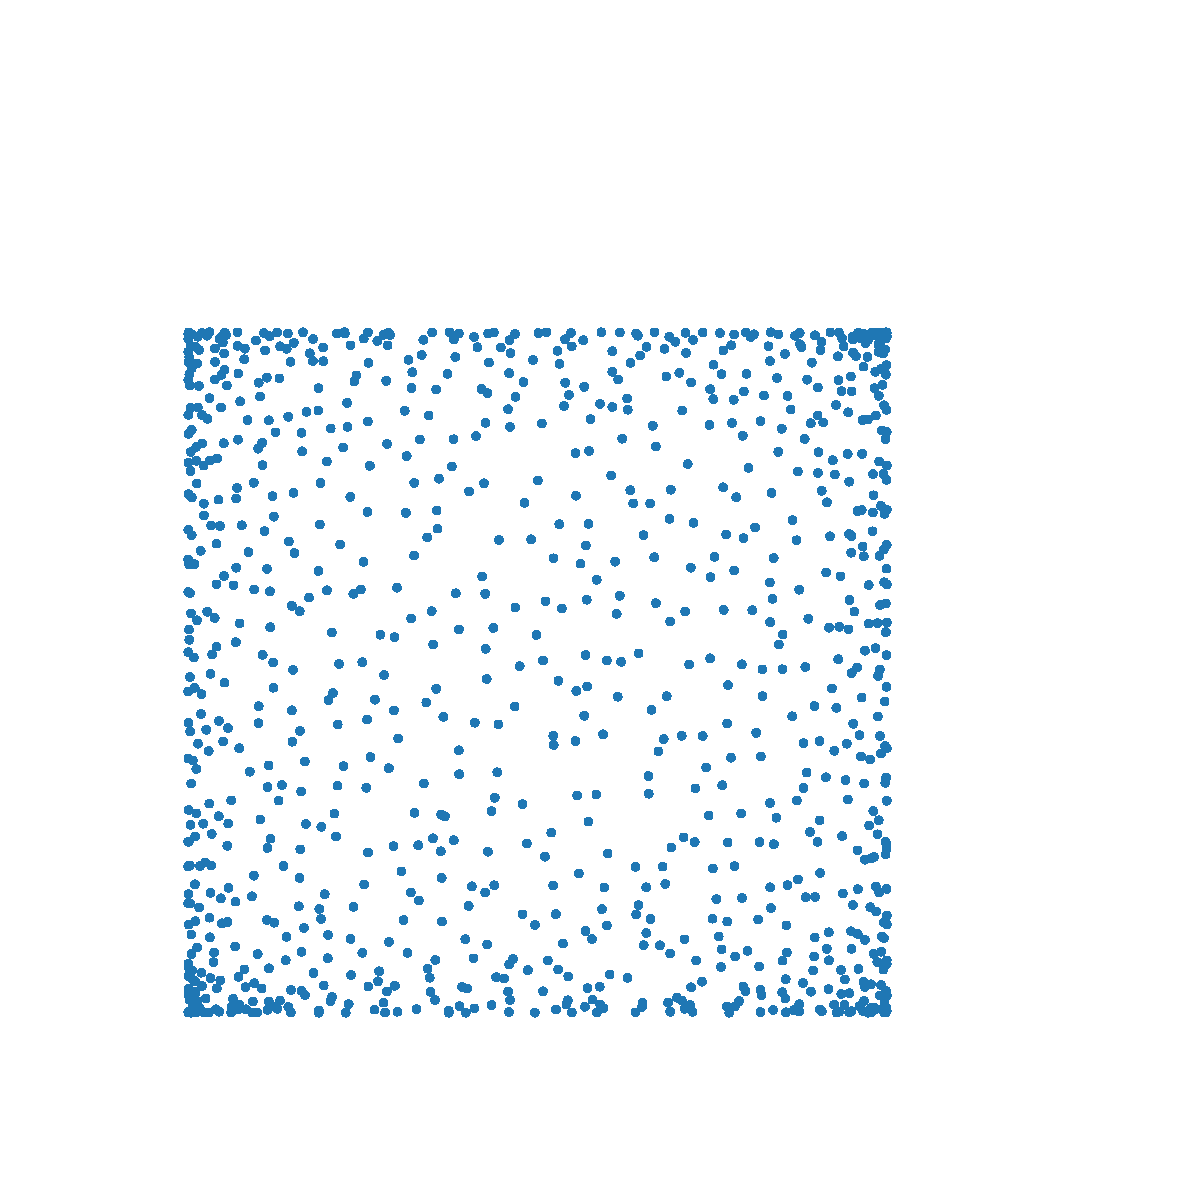
\includegraphics[height=10.5em]{images/multivariate_jacobi_2D_1000points.pdf}
            \label{fig:2D_jacobi_sample}
        }
%            \includegraphics[height=10.5em]{../img/bolt_volumes.pdf}
        % \qquad\qquad
        \subfigure[$\beta=2$-Laguerre ensemble]{
            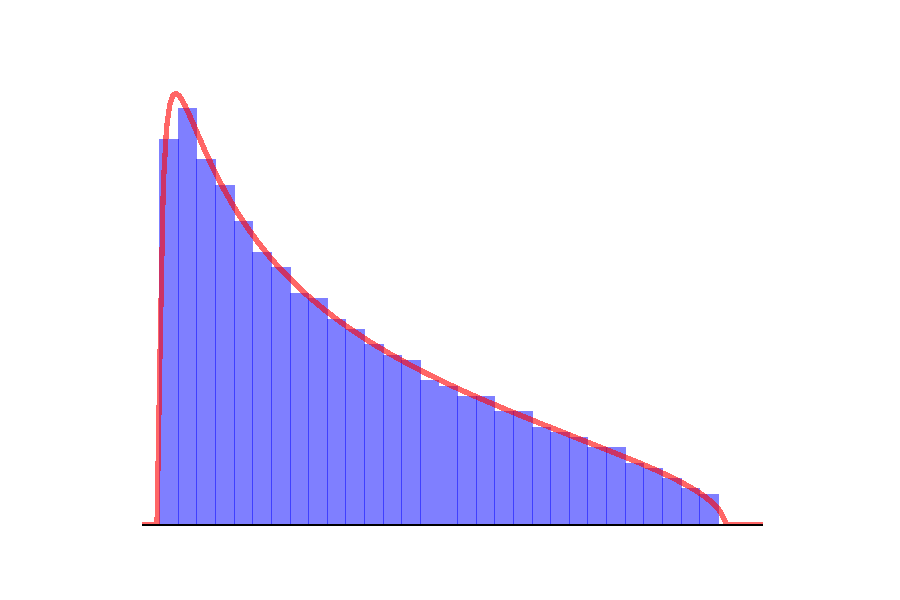
\includegraphics[height=10.5em]{images/LUE.pdf}
            \label{fig:LUE}
        }
        \subfigure[$\bfK$ kernel of UST]{
            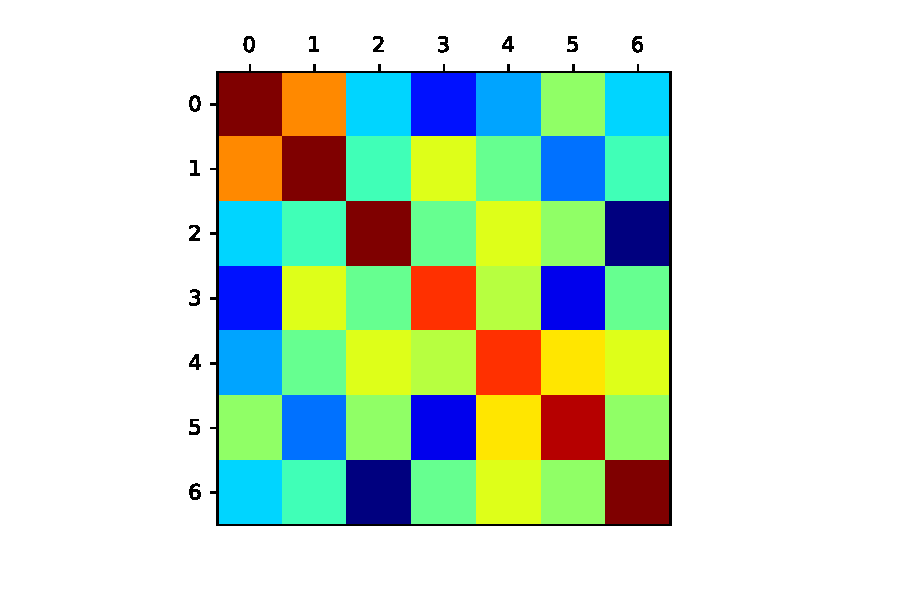
\includegraphics[height=10.5em]{images/UST_kernel.pdf}
            \label{fig:UST_kernel}
        }
        \vspace{-0.75em}
        \caption{Some displays available in \DPPy}
        \label{fig:DPPy_figs}
        \vspace{-10em}
    \end{figure*}

% section the_dppy_toolbox (end)

% \section{Conclusion and future work} % (fold)
% \label{sec:conclusion_and_future_work}

% section conclusion_and_future_work (end)

% Acknowledgements should go at the end, before appendices and references
%\newpage
%{\small
\clearpage

\acks{%
We would like to thank \href{https://guillep.github.io/}{Guillermo Polito} for leading our reproducible research \href{https://github.com/CRIStAL-PADR/reproducible-research-SE-notes}{workgroup}, this project owes him a lot.
We acknowledge funding by European CHIST-ERA project DELTA, the French Ministry of Higher Education and Research, the Nord-Pas-de-Calais Regional Council, Inria and Otto-von-Guericke-Universit\"at Magdeburg associated-team north-European project Allocate, and French National Research Agency projects ExTra-Learn (n.ANR-14-CE24-0010-01) and BoB (n.ANR-16-CE23-0003).
}

% Manual newpage inserted to improve the layout of sample file - not
% needed in general before the appendices/bibliography.

% \newpage

% \appendix
% \section*{Appendix A.}
% \label{app:theorem}

% Note: in this sample, the section number is hard-coded in. Following
% proper LaTeX conventions, it should properly be coded as a reference:

%In this appendix we prove the following theorem from
%Section~\ref{sec:textree-generalization}:

% \vskip 0.2in

\bibliography{biblio_new}

\end{document}
